\documentclass[11pt]{beamer}
\usepackage[utf8]{inputenc}
%\usepackage[english]{babel}
\usepackage[czech]{babel}
\usepackage[T1]{fontenc}
\usepackage{amsmath}
\usepackage{amsthm}
\usepackage{amssymb}
\usepackage{amstext}



\usetheme		{Frankfurt}%,Malmoe,Warsaw,3kolonky:CambridgeUS,Madrid %%Ilmenau,Antibes,,,,Luebeck,Copenhagen,
%\beamertemplateballitem
\usecolortheme	{beaver}%crane, orchid

\author{Bc. Jan Kučera}
%\title{Rényi decomposable minimum distance estimators and signal separation through divergence decision trees}
\title{Vývoj a testování nových statistických technik pro separaci signálů z rozpadových procesů ve Fermilabu}
%\institute{FNSPE, CTU \\ $\quad$ $\quad$ $\quad$ \\ Work supervisor: Ing. Václav Kůs Ph.D.}
\institute{FJFI, ČVUT\\ $\quad$ $\quad$ $\quad$ \\ Vedoucí práce: Ing. Václav Kůs Ph.D.}
\date{29.4.2013}

\newcommand{\intpa}{\int p_\theta^{1+\alpha}(x) \, \mathrm{d}x }
\newcommand{\fn}{\frac{1}{n} \sum_{i=1}^n p_{\theta}^{\alpha}\left( x_i \right)}
\newcommand{\fln}{\frac{1}{n} \sum_{i=1}^n \ln p_{\theta}\left( x_i \right)}
\newcommand{\Cat}{C_\alpha\left( \theta \right)}
\newcommand{\amtiT}{\arg \max_{\theta \in \Theta}}
\newcommand{\fa}{\frac{\alpha}{1+\alpha}}
\newcommand{\dzero}{D$\emptyset$ }
\newcommand{\ttbar}{$t\bar{t}$ }


\begin{document}
\setbeamertemplate{navigation symbols}{}%remove navigation symbols
\begin{frame}
	\maketitle
\end{frame}

%\begin{frame}{Table of contents} %outline
\begin{frame}{Obsah}
    	\tableofcontents
\end{frame}

%
%\begin{frame}
%	Let $\mathcal{P} = \lbrace P_\theta : \theta \in \Theta \subset \mathbb{R}^m \rbrace$ be set of probability measures on $\left(\mathcal{X},\mathcal{A}\right)$. \\
%	Let $Q$ probability measure on $\left(\mathcal{X},\mathcal{A}\right)$. \\
%	Let $X_1,\ldots,X_n$ be i.i.d observations governed by convex mixtures $\tilde{P} = (1-\epsilon) P_\theta + \epsilon Q$. We denote $\mathcal{\tilde{P}} = \mathcal{P} \cup \lbrace \tilde{P} \rbrace$
%\end{frame}

\begin{frame}
Motivace
\begin{enumerate}


\item studium robustních Rényiho divergencí
\item výběr vhodných proměnných pro separaci vysoko-dimenzionálních fyzikálních dat z částicového urychlovače ve Fermilabu
\begin{itemize}
	\item dobrá shoda mezi Monte Carlo simulacemi a daty
	\item rozdíly mezi signálem a ostatními kanály
\end{itemize}
\item použití divergencí pro samotnou separaci v divergenčních rozhodovacích stromech
\end{enumerate}
\end{frame}

\section{Rényiho pseudovzdálenosti} %******************************************** RENYI PSEUDO-DISTANCE
\begin{frame}{Rényiho rozložitelné pseudovzdálenosti}
\begin{theorem}[Minimální odhad s Rényiho pseudovzdáleností]
Nechť pro nějaké $\beta>0$ platí
	\begin{equation*}
		p^\beta, q^\beta,\ln{p} \in \mathrm{L}_1(Q), \quad \forall P \in \mathcal{P}, Q \in \mathcal{\tilde{P}}.
	\end{equation*}
	Potom pro každé $\alpha$, $0 < \alpha \leq \beta\;$ platí
{\footnotesize
\begin{align*}
 \mathcal{R}_\alpha (P,Q) = & \ln{\left( \int{p^\alpha \mathrm{d}P } \right)^{\frac{1}{1+\alpha}}} + 
						\ln{\left( \int{q^\alpha \,\mathsf{d}Q } \right)^{\frac{1}{\alpha (1+\alpha)}}} 
						& - \ln{\left( \int{p^\alpha \,\mathsf{d}Q } \right)^{ \frac{1}{\alpha}}}
\end{align*}}definuje třídu rozložitelných pseudovzdáleností %\cite{Decomposable2011}
(nepožadujeme trojúhelníkovou nerovnost ani symetrii).
\end{theorem}
\pause
\begin{itemize}
\item pro často používaná rozdělení není $\beta$ nijak omezené
\end{itemize}
\end{frame}

\begin{frame}
\begin{itemize}
\item odhadujeme parametry rozdělení $P$
\item minimalizujeme pouze {\color{red}členy} obsahující hustotu $p$ 
\end{itemize}

{\footnotesize
\begin{align*}
 			\mathcal{R}_\alpha (P,Q) = & \; {\color{red}\ln{\left( \int{p^\alpha \,\mathsf{d}P } \right)^{\frac{1}{1+\alpha}}}} + 
						\ln{\left( \int{q^\alpha \,\mathsf{d}Q } \right)^{\frac{1}{\alpha (1+\alpha)}}} 
						& {\color{red} - \ln{\left( \int{p^\alpha \,\mathsf{d}Q } \right)^{ \frac{1}{\alpha}}}}
\end{align*}}
\begin{itemize} 
\item pokud je $Q$ empirická distribuce, prostřední člen závisí pouze na datech
\pause
\item rychlý vypočet pro normální, cauchyho, exponenciální, laplaceovo, weibullovo rozdělení
\item pro $\alpha = 0$ přechází odhad v MLE 
\item odhady robustní outlierům se zvyšujícím se $\alpha$

\end{itemize}
\end{frame}

%\begin{frame}
%If we replace Q by the empirical distribution $P_n$, we get
%\begin{equation*}
%	\theta_{\mathcal{R}_\alpha,n} = 
%	\begin{cases}
%		\displaystyle{ \amtiT \left( \intpa \right)^{-\frac{\alpha}{1+\alpha}} \fn }, \\
%		\qquad \text{for } 0 < \alpha \leq \beta, \\
%		\displaystyle{ \amtiT  \fln },\\
%		\qquad \text{for } \alpha = 0.
%	\end{cases}	
%\end{equation*}
%	So for $\alpha = 0 $ the $\theta_{\alpha,n} = \theta_{MLE}$
%\end{frame}

\begin{frame}{Influenční funkce} % --------------- Influence function

{\footnotesize Míra závislosti odhadů na jednotlivých pozorováních }
%{\footnotesize\[\mathrm{IF}(x;T_{\mathcal{R}_\alpha},\mu) = (1+\alpha )^{\frac{3}{2}} (x-\mu )  e^{-\frac{\alpha}{2} (x-\mu )^2}\]}
%{\footnotesize\[\mathrm{IF}(x;T_{\mathcal{R}_\alpha},\lambda) = (1 + \alpha)^2 \left(-\lambda + (1 + \alpha)|x|\right)  e^{-\frac{\alpha|x|}{\lambda}}\]}
\vspace*{-0.1in}	
\begin{figure}[htb]
\begin{tabular}{cc}
	\includegraphics[width=1.8in]{Normal-IF-mu.pdf}
	&
	\includegraphics[width=1.8in]{Normal-IF-lambda-eps-converted-to.pdf}
	\\
	{\footnotesize $\mathrm{IF}(x;T_{\mathcal{R}_\alpha},\widehat{\mu} = 0) $, $\sigma = 1$}
	&
	{\footnotesize $\mathrm{IF}(x;T_{\mathcal{R}_\alpha},\widehat{\sigma} = 1)$, $\mu = 0$}
	\\
\end{tabular}
\end{figure}
\vspace*{-0.1in}	
{\footnotesize Pro $\alpha> 0$ :}
\begin{itemize}
	\item {\footnotesize IF je omezená $\rightarrow$ B-robustní}
	\item {\footnotesize$\lim_{x\rightarrow \infty} \mathrm{IF}(x;T_{\mathcal{R}_\alpha},\cdot) = 0 \; \rightarrow$ robustní vůči outlierům}
\end{itemize}
\end{frame}

\section{Heuristický přístup} % ---------------------------- Heuristic approach
\begin{frame}{Vzdálenost v parametrickém prostoru}
\begin{itemize}
\item $\varepsilon$-znečištěné rozdělení
\end{itemize}

	\[ \mathcal{R}_\alpha(P,Q), \; \alpha = 0.7\]
	\[ \text{data: }(1-\varepsilon)\mathrm{N}(0,1) + \varepsilon \mathrm{N}(0,10), \; \varepsilon =  0.2 \]
\begin{center}
	\vspace{-0.3in}
	\begin{figure}[htb]
	\begin{tabular}{cc}
		\includegraphics[width = 5.4cm]{Renyi-0,7_K-1_n-20_eps-0,20_N0,1-N0,10,dist.png}			
		&
		\includegraphics[width = 5.4cm]{Renyi-0,7_K-1_n-500_eps-0,20_N0,1-N0,10,dist.png}
		\\
		{\footnotesize $n = 20$}
		&
		{\footnotesize $n = 500$}	
		
	\end{tabular}
	\end{figure}
	\end{center}
    $\;$\\$\;$\\
\end{frame}


\begin{frame}
	Malé datové vzorky kombinované s volbou "robustního"  $\:\alpha \gg 0$ 
		\vspace{-0.2in}
		\begin{figure}[htb]
		\begin{tabular}{cl}		
		\includegraphics[width = 5.4cm]{Renyi-0,7_K-1_n-20_eps-0,20_N0,1-N0,10,dist.png}				&
		\includegraphics[width = 5.0cm]{Normal-IF-lambda-eps-converted-to.pdf}		
		%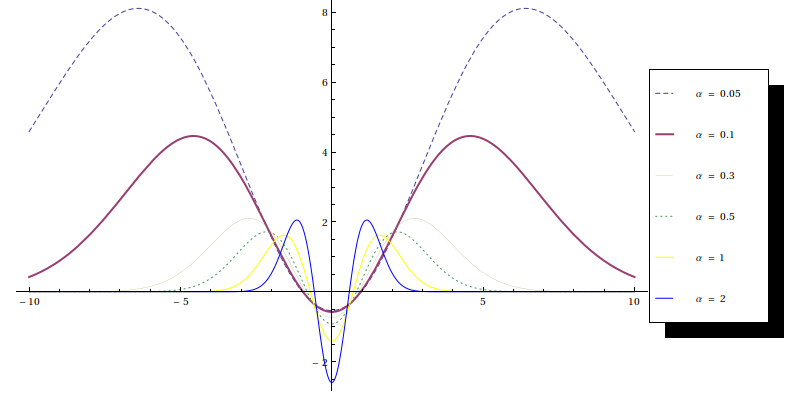
\includegraphics[width = 5.2cm]{IF-Normal-sigma.png}
		\end{tabular}
		\end{figure}
		\begin{itemize}
		\item $\mathcal{R}_{\alpha\gg 0}$ preferuje $\delta-$funkce ($\sigma \rightarrow 0$) 
		\item hledáme model popisující celý datový vzorek
		\end{itemize}
	
\end{frame}

\begin{frame}{Heuristika}
\begin{itemize}
\item konvoluce funkce vzdáleností s vyhlazovací maskou o malé velikosti
\item gaussovská a konstantní maska mají velmi podobné výsledky
\end{itemize}
    \vspace{-0.3in}
	\begin{figure}[htb]
	\begin{tabular}{cc}
		\includegraphics[width = 5.5cm]{heurRenyi.pdf}
		&
		\includegraphics[width = 5.4cm]{heurAverage.pdf}			
		\\
		{\footnotesize Rényiho vzdálenost}
		&
		{\footnotesize Rényiho vzdálenost po vyhlazení}	
		
	\end{tabular}
	\end{figure}
	\pause
	algoritmus
	\begin{enumerate}
	\item minimalizujeme heuristickou funkci
	\item pak minimalizujeme klasickou Rényiho vzdálenost
	\end{enumerate}

\end{frame}

\section{Analýza dat z Fermilabu}
\begin{frame}{Data z detektoru \dzero}
	\vspace{-0.3in}
	\begin{figure}
	\includegraphics[width=0.75\textwidth]{dataFnal.pdf}
	\caption{\footnotesize První a druhá hlavní komponenta části analyzovaných dat}
	\end{figure}
	\vspace{-0.2in}
\begin{itemize}
	\item vysoko-dimenzionální data 
	\begin{itemize}
	\item z detektoru až 600 proměnných
	\item pro analýzy 20 - 50 proměnných
	\end{itemize}
\end{itemize}\end{frame}

\begin{frame}
Výběr proměnných pro separaci
\begin{itemize}
\item dobrá shoda Monte Carlo simulací a dat
\begin{itemize}
\item testy dobré shody
\item pořadí odvozené z divergenčních vzdáleností
\end{itemize}
\item velká diference mezi signálem a ostatními kanály
\begin{itemize}
\item pořadí odvozené z divergenčních vzdáleností
\end{itemize}
\end{itemize}
\end{frame}

\begin{frame}{Použité statistiky}

\begin{tabular}{l l}
Kolmogorov-Smirnov: & $\sup |F_m(X_i) - G_n(X_i)|$ \vspace{0.1in}\\
Cramér-von Mises: & $ \sum_{i=1}^{m+n} \left( F_m\left(X_i\right) -
G_n\left(X_i\right)\right)^2$ \vspace{0.1in}\\

Anderson-Darling: & $\sum_{i=1}^{m+n} \dfrac{\left( F_m\left(X_i\right) -
G_n\left(X_i\right)\right)^2}{H_{m+n}\left( 1 - H_{m+n} \right)}$ \vspace{0.1in}\\
Rényi: & $\log \sum_{i=1}^{\tilde{n}} \hat{f}_i^\alpha \hat{g}_i^{1-\alpha}$ 
\end{tabular}

\pause
\begin{itemize}
	\item velké množství dat $\rightarrow$ limitní rozdělení
	\item Rényiho vzdálenost počítaná na histogramech $\rightarrow$ problém s počtem binů
\end{itemize}
\end{frame}


  \begin{frame}{Kolmogorov-Smirnov, Cramér, Anderson-Darling}
    \vspace{-.2cm}
    \begin{center}
      \begin{tabular}{cc}{\footnotesize}
%	\includegraphics[width=0.3\textwidth]{./figs/KS_cr_AD-ele-njet_2.pdf}&  
	\includegraphics[width=0.39\textwidth]{./figs/KS_cr_AD-ele-njet_3.pdf}& 
	\includegraphics[width=0.39\textwidth]{./figs/KS_cr_AD-ele-njet_4.pdf}\\
%	\footnotesize electron 2 jets&
	\footnotesize electron 3 jets&
	\footnotesize electron 4 jets\\
%	\includegraphics[width=0.3\textwidth]{./figs/KS_cr_AD-muo-njet_2.pdf}&
	\includegraphics[width=0.39\textwidth]{./figs/KS_cr_AD-muo-njet_3.pdf}&
	\includegraphics[width=0.39\textwidth]{./figs/KS_cr_AD-muo-njet_4.pdf}\\
%	\footnotesize muon 2 jets&
	\footnotesize muon 3 jets&
	\footnotesize muon 4 jets
      \end{tabular}
    \end{center}
  \end{frame}
  
  \begin{frame}{Rényiho histogramy}
    \vspace{-.2cm}
    \begin{center}
      \begin{tabular}{cc}{\footnotesize}
%	\includegraphics[width=0.3\textwidth]{./figs/Rhist-ele-njet_2.pdf}&  
	\includegraphics[width=0.39\textwidth]{./figs/Rhist-ele-njet_3.pdf}& 
	\includegraphics[width=0.39\textwidth]{./figs/Rhist-ele-njet_4.pdf}\\
%	\footnotesize electron 2 jets&
	\footnotesize electron 3 jets&
	\footnotesize electron 4 jets\\
%	\includegraphics[width=0.3\textwidth]{./figs/Rhist-muo-njet_2.pdf}&
	\includegraphics[width=0.39\textwidth]{./figs/Rhist-muo-njet_3.pdf}&
	\includegraphics[width=0.39\textwidth]{./figs/Rhist-muo-njet_4.pdf}\\
%	\footnotesize muon 2 jets&
	\footnotesize muon 3 jets&
	\footnotesize muon 4 jets
      \end{tabular}
    \end{center}
  \end{frame}
  
  \begin{frame}{Rényiho vzdálenost včetně jádrového odhadu}
    \vspace{-.2cm}
    \begin{center}
      \begin{tabular}{cc}{\footnotesize}
%	\includegraphics[width=0.3\textwidth]{./figs/Rall-ele-njet_2.pdf}&  
	\includegraphics[width=0.39\textwidth]{./figs/Rall-ele-njet_3.pdf}& 
	\includegraphics[width=0.39\textwidth]{./figs/Rall-ele-njet_4.pdf}\\
%	\footnotesize electron 2 jets&
	\footnotesize electron 3 jets&
	\footnotesize electron 4 jets\\
%	\includegraphics[width=0.3\textwidth]{./figs/Rall-muo-njet_2.pdf}&
	\includegraphics[width=0.39\textwidth]{./figs/Rall-muo-njet_3.pdf}&
	\includegraphics[width=0.39\textwidth]{./figs/Rall-muo-njet_4.pdf}\\
%	\footnotesize muon 2 jets&
	\footnotesize muon 3 jets&
	\footnotesize muon 4 jetsg
      \end{tabular}
    \end{center}
  \end{frame}

\begin{frame}{Závěr}
\begin{itemize}
\item Odvodili vzorce pro rychlý výpočet Rényiho pseudovzdáleností pro odhady
\item Byla navržena a testována heuristika pro velmi robustní odhad na malých datových vzorcích
\item Použity některé divergence metriky pro výběr vhodných proměnných pro separaci fyzikálních dat
\end{itemize}
\end{frame}

%\begin{frame}{Divergence Decision Tree}
%    \vspace{-0.45in}
%	\begin{figure}[htb]
%	\begin{flushright}
%		\includegraphics[width = 3cm]{myDDT.png}			
%	\end{flushright}
%	\end{figure}
%
%	\vspace{-0.6in}
%%	$D_\alpha(A_1) = \min_Q \sum_{x \in A_1} D_\alpha(p_x\Vert Q)$ \\
%	Algorithm:
%	\begin{itemize}
%	\item find node with max $D_\alpha(S)$:
%	\begin{itemize}
%		\item subset of parameters is chosen via PCA
%		\item all pairs of parameters are chosen from this subset and
% 		\item partition $(A_1,A_2)$ of set $S$ is found such, that $D_\alpha(A_1) + D_\alpha(A_2)$ is minimized
% 		\begin{itemize}
% 			\item $D_\alpha(A_1) = \min_Q \sum_{x \in A_1} D_\alpha(p_x\Vert Q)$
% 		\end{itemize}
%		\item equivalently $\frac{n_1}{n}D_\alpha(A_1\Vert S) + \frac{n_2}{n}D_\alpha(A_2\Vert S)$ is minimized%\cite{DDT}
%	\end{itemize}
%	\end{itemize}
%%	\begin{itemize}
%%	\item 
%%		${33 \choose 2}  = 528$, but for subset of 15 principal components, we have ${15 \choose 2}  = 105$
%%	\end{itemize}	
%\end{frame}

%\begin{frame}{Maximization vs. minimization}
%Maximization of $\frac{n_1}{n}D_\alpha(A_1\Vert S) + \frac{n_2}{n}D_\alpha(A_2\Vert S)$
%	\begin{itemize}
%		\item chooses the partitioning which takes the most different distributions 
%	\end{itemize}
%Minimization of $D_\alpha(A_1) + D_\alpha(A_2)$
%	\begin{itemize}
%		\item chooses the partitioning which chooses the distributions having the smallest divergence
%	\end{itemize}
%
%\end{frame}
%
%\begin{frame}{Unsupervised learning}
%	\begin{itemize}
%		\item method is originally designed for unsupervised learning
%		\item we had to label the final nodes:
%		\begin{itemize}
%			\item data for classification are separated via DDT together with Training set
%			\item nodes are labelled according to Training data they contain
%		\end{itemize}
%		\item data are too complex for unsupervised methods \\
%		\end{itemize}
%		Relative frequency of signal in each leaf node: \\ 
%		{\scriptsize$P_S = (0.17, 0.28,  0.41, 0.06, 0.30, 0, 0.33, 0.04, 0.44, 0.14, 0.03, 0.30, 0.17, 0.33)$}\\ \mbox{ } \\
%$\Rightarrow$	Teacher has to be incorporated to the method
%\end{frame}


%\begin{frame}{Suggestions for supervised learning}
%	\begin{itemize}
%		\item use of supervised clustering method in the step of dividing node
%		\begin{itemize}
%			\item model based clustering
%			\item support vector machine
%		\end{itemize}
%		\item creating a sequence of {\em boosted} trees
%		\begin{itemize}
%			\item each falsely classified date would gain weight to the next iteration
%		\end{itemize}
%%		\item this approach 'counters' the idea of sequencing primitive classifiers into strong one
%	\end{itemize}
%\end{frame}

%\section*{$\,$}
%\begin{frame}
%\begin{thebibliography}{10}
%
%%\bibitem{Antoch92}Antoch, J., Vorlíčková, D., {\em Vybrané metody statistické analýzy dat}, Academia, Praha, 1992
%%\bibitem{Basu}Basu, A., Harris, I.R., Hjort, N.L., Jones M.C. {\em Robust and efficient estimation by minimising a density power divergence}, Biometrika, 85, 549-559, 1998
%\bibitem{Decomposable2011}Broniatowski, M., Toma, A., Vajda, I. {\em Decomposable pseudo-distances and Applications in Statistical Estimation}, arXiv:1104.1541v1, 2011
%%\bibitem{Vajda2009}Broiatowski, M.,Vajda, I. {\em Several Aplications of Divergence Criteria in Continuous Families}, Research report No 2257 September 2009, ÚTIA AV Č%R, Praha, 2009
%%\bibitem{Demut2010}Demut, R.{\em Robust properties of minimum divergence density estimators}, Diplomová práce, ČVUT, Praha, 2010
%%\bibitem{Lecuyer}L'Ecuyer, P. {\em Efficient and Portable Combined Random Number Generators}, Communications of the ACM, 1988
%%\bibitem{LieseVajde}Liese, F., Vajda, I. {\em On Divergences and Informations in Statistics and Information Theory}, IEEE Transactions on Information Theory, Vol. 52, No. 10, 2006, s.4394-4412
%%\bibitem{Vajda1995}Vajda, I. {\em Information - Theoretic Methods in Statistics}, Research report No 1834 March 1995, ÚTIA AV ČR, Praha, 1995
%%\bibitem{Virius98}Virius, M. {\em Aplikace matematické statistiky, metoda Monte Carlo}, ČVUT, Praha, 1998
%\bibitem{DDT}Karakos, D., Khudanpur, S., Marchette D. J., Papamarcou A., Priebe C. E. {\em On the minimization of concave information functionals for unsupervised classification via decision trees}, Statistics and Probability Letters 78, 2008
%
%\end{thebibliography}
%\end{frame}

\begin{frame}
	\begin{center}
		Děkuji za pozornost.
	\end{center}
\end{frame}

\end{document}
